\documentclass[letterpaper,11pt]{article}

\usepackage{latexsym}
\usepackage[empty]{fullpage}
\usepackage{titlesec}
\usepackage{marvosym}
\usepackage[usenames,dvipsnames]{color}
\usepackage{verbatim}
\usepackage{enumitem}
\usepackage[hidelinks]{hyperref}
\usepackage{fancyhdr}
\usepackage[english]{babel}
\usepackage{tabularx}
\usepackage{fontawesome5}
\usepackage{multicol}
\setlength{\multicolsep}{-3.0pt}
\setlength{\columnsep}{-1pt}
\input{glyphtounicode}

%new packages

\usepackage{fontenc}
\usepackage{amsmath}
\usepackage{amssymb}
\usepackage{graphicx}



%----------FONT OPTIONS----------

\pagestyle{fancy}
\fancyhf{} % clear all header and footer fields
\fancyfoot{}
\renewcommand{\headrulewidth}{0pt}
\renewcommand{\footrulewidth}{0pt}

% Adjust margins
\addtolength{\oddsidemargin}{-0.6in}
\addtolength{\evensidemargin}{-0.5in}
\addtolength{\textwidth}{1.19in}
\addtolength{\topmargin}{-.7in}
\addtolength{\textheight}{1.4in}

\urlstyle{same}

\raggedbottom
\raggedright
\setlength{\tabcolsep}{0in}

% Sections formatting
\titleformat{\section}{
  \vspace{-4pt}\scshape\raggedright\large\bfseries
}{}{0em}{}[\color{black}\titlerule \vspace{-5pt}]



% Ensure that generate pdf is machine readable/ATS parsable
\pdfgentounicode=1

%-------------------------
% Custom commands
\newcommand{\resumeItem}[1]{
  \item\small{
    {#1 \vspace{-2pt}}
  }
}

\newcommand{\classesList}[4]{
    \item\small{
        {#1 #2 #3 #4 \vspace{-2pt}}
  }
}

\newcommand{\resumeSubheading}[4]{
  \vspace{-2pt}\item
    \begin{tabular*}{1.0\textwidth}[t]{l@{\extracolsep{\fill}}r}
      \textbf{#1} & \textbf{\small #2} \\
      \textit{\small#3} & \textit{\small #4} \\
    \end{tabular*}\vspace{-7pt}
}

\newcommand{\resumeSubSubheading}[2]{
    \item
    \begin{tabular*}{0.97\textwidth}{l@{\extracolsep{\fill}}r}
      \textit{\small#1} & \textit{\small #2} \\
    \end{tabular*}\vspace{-7pt}
}

\newcommand{\resumeProjectHeading}[2]{
    \item
    \begin{tabular*}{1.001\textwidth}{l@{\extracolsep{\fill}}r}
      \small#1 & \textbf{\small #2}\\
    \end{tabular*}\vspace{-7pt}
}


\newcommand{\resumeSubItem}[1]{\resumeItem{#1}\vspace{-4pt}}

\renewcommand\labelitemi{$\vcenter{\hbox{\tiny$\bullet$}}$}
\renewcommand\labelitemii{$\vcenter{\hbox{\tiny$\bullet$}}$}

\newcommand{\resumeSubHeadingListStart}{\begin{itemize}[leftmargin=0.0in, label={}]}
\newcommand{\resumeSubHeadingListEnd}{\end{itemize}}
\newcommand{\resumeItemListStart}{\begin{itemize}}
\newcommand{\resumeItemListEnd}{\end{itemize}\vspace{-5pt}}


\begin{document}
\fontfamily{cmr}\selectfont
\begin{center}
\parbox{3.0cm}{%
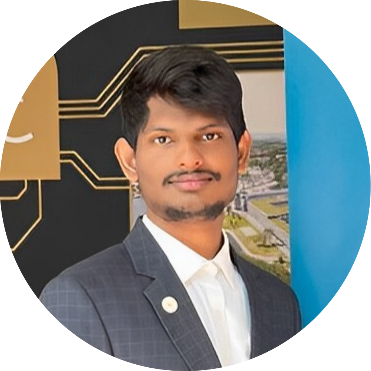
\includegraphics[width=2.7cm,clip]{images/resume_pic_m.png}}
}
\parbox{\dimexpr\linewidth-3.8cm\relax}{
\vspace{-20pt}
\begin{tabularx}{\linewidth}{L r} \\
    {\Huge \scshape  Venkata Sai Yakkshit Reddy Asodi}~
    \href{https://www.cedzlabs.com/yakkshit}{\vspace{1pt}}\\
      Geneva, Switzerland \\ \vspace{1pt}
     \small \raisebox{-0.1\height}\faPhone\ +91 9493006444 ~ \href{mailto:saiyakkshit2001@gmail.com}{\raisebox{-0.2\height}\faEnvelope\  {saiyakkshit2001@gmail.com}} ~ 
    \href{https://linkedin.com/in/yakkshit/}{\raisebox{-0.2\height}\faLinkedin\ {yakkshit}}  ~
    \href{https://yakkshit.com/}{\raisebox{-0.2\height}\faGlobe\ {yakkshit.com}}  ~
    \href{https://github.com/yakkshit}{\raisebox{-0.2\height}\faGithub{ yakkshit}}
    \vspace{-8pt}
\end{tabularx}
}
\end{center}

\vspace{-23pt}
\href{https://www.yakkshit.com/#details}{\section{Summary \faLink}
Full Stack Developer with strong expertise in data-driven applications and visualization. Experienced in developing automated systems using Python and modern web technologies. Proven track record in creating efficient backend processes and user-friendly interfaces. Skilled in SQL, API development, and implementing machine learning solutions. Strong background in agile methodologies and cross-functional team collaboration.}

\section{\href{https://www.linkedin.com/in/yakkshit/details/skills/}{Technical Skills} \faLink}
\begin{itemize}[leftmargin=0.15in, label={}]
\small{\item{
\textbf{Languages \& Frontend - }{Python, JavaScript, HTML5, CSS3, Plotly} \\
\textbf{Data \& ML - }{SQL, Pandas, NumPy, Scikit-learn, Databricks} \\
\textbf{Backend \& APIs - }{REST APIs, Flask/Django, Database Design} \\
\textbf{Tools \& Practices - }{Git, Jira, Unit Testing, Agile/Scrum}\\
}}
\end{itemize}
\vspace{-10pt}

\section{Experience \faLinkedin}
\resumeSubHeadingListStart

\resumeSubheading
{\large Circleup AG \faBuilding}{December 2023 -- July 2024}
{Full Stack Developer}{\faMapMarker \hspace{0.1cm} Zurich, Switzerland}\\
\vspace{10pt}
\textbf{Responsibilities:}
\resumeItemListStart
\vspace{-10pt}
\resumeItem{Developed data visualization dashboards using Plotly and JavaScript, improving process monitoring efficiency by 40\%}
\resumeItem{Implemented automated data processing pipelines using Python (Pandas, NumPy) reducing manual data handling time by 65\%}
\resumeItem{Created RESTful APIs for seamless integration between frontend and backend systems, handling 1M+ daily requests}
\resumeItemListEnd
\vspace{-3pt}
\textbf{Environment:}\emph{Python, JavaScript, SQL, Plotly, Pandas, REST APIs}

\resumeSubheading
{Cedzlabs \faBuilding}{March 2023 -- November 2023}
{Software Developer}{\faMapMarker \hspace{0.1cm} Zurich, Switzerland}\\
\vspace{10pt}
\textbf{Responsibilities:}
\vspace{-10pt}
\resumeItemListStart
\resumeItem{Built machine learning pipelines using scikit-learn for predictive maintenance, achieving 90\% accuracy}
\resumeItem{Developed and maintained comprehensive API documentation, reducing onboarding time for new team members by 50\%}
\resumeItemListEnd
\vspace{-3pt}
\textbf{Environment:}\emph{Python, Scikit-learn, SQL, Git, Jira}

\section{Projects \faGithub}
\vspace{-5pt}
\resumeSubHeadingListStart
\resumeProjectHeading
{\textbf{\href{https://ui.cedzlabs.com/resume}{Manufacturing Analytics Platform}} $|$ \emph{Python, Plotly, SQL}}{2024}\\
\vspace{6pt}
\textbf{Description:}
\vspace{-5pt}
\resumeItemListStart
\resumeItem{Developed a comprehensive analytics platform for manufacturing process optimization. Implemented interactive dashboards using Plotly for real-time monitoring, integrated machine learning models for predictive maintenance, and created automated reporting systems. Reduced process inefficiencies by 35\% through data-driven insights.}
\resumeItemListEnd
\vspace{4pt}
\textbf{Tools:}\emph{
Python, Plotly, SQL, Pandas, Scikit-learn, Flask}
\vspace{-10pt}

\resumeProjectHeading
{\href{https://yakkshit.com}{\textbf{Automated Recommendation System}} $|$ \emph{Python, ML, APIs}}{2023}\\
\vspace{6pt}
\textbf{Description:}
\vspace{-5pt}
\resumeItemListStart
\resumeItem{Built an ML-powered recommendation system for process optimization. Implemented RESTful APIs for data access, created visualization tools for performance monitoring, and developed automated testing suite achieving 95\% coverage.}
\resumeItemListEnd
\vspace{4pt}
\textbf{Tools:}\emph{Python, scikit-learn, REST APIs, Pytest}
\vspace{-12pt}

\section{Achievements / Technical Expertise}
\resumeSubHeadingListStart
\resumeItemListStart
\resumeItem{Reduced system processing time by 70\% through optimization of SQL queries and data pipelines}
\resumeItem{Implemented automated testing framework achieving 95\% code coverage}
\resumeItem{Successfully delivered 3 major projects in agile environment using Jira for project tracking}
\resumeItemListEnd

\resumeSubHeadingListEnd
\textbf{Methodologies:}\emph{Agile Development, Test-Driven Development, CI/CD} \\
\textbf{Education:}\emph{Bachelor of Technology in Computer Science, Bth Sweden (2019-2023)} \\
\textbf{Languages:}\emph{English - Fluent $|$ German - A1 Level}

\vspace{10pt}
\end{document}